\documentclass[12pt]{article}
\usepackage{tikz}
\usepackage{amsmath}
% Underlining package
\usepackage{ulem}
\usetikzlibrary{angles,quotes}
\usetikzlibrary{intersections}
\usetikzlibrary{arrows.meta}
\usetikzlibrary{calc}
\usepackage[a4paper, portrait, margin=1cm]{geometry}
\usepackage{fancyhdr}

\def \HeadingQuestions {\section*{\Large Name: \underline{\hspace{8cm}} \hfill Date: \underline{\hspace{3cm}}} \vspace{-3mm}
{Parallel lines Angles: Questions} \vspace{1pt}\hrule}

% raise footer with page number; no header
\fancypagestyle{myfancypagestyle}{
  \fancyhf{}% clear all header and footer fields
  \renewcommand{\headrulewidth}{0pt} % no rule under header
  \fancyfoot[C] {\thepage} \setlength{\footskip}{6pt} % raise page number 6pt
}
\pagestyle{myfancypagestyle}  % apply myfancypagestyle

\newcounter{minipagecount}

\begin{document}
\HeadingQuestions
\vspace{8mm}

\begin{minipage}{0.75\textwidth}
  \refstepcounter{minipagecount}
  \noindent{(\theminipagecount)}\quad
  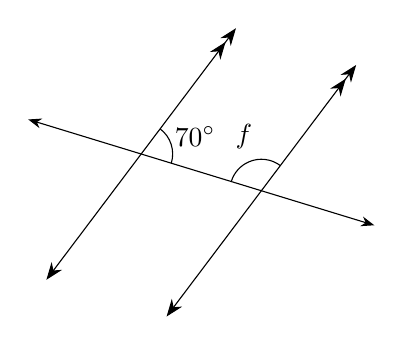
\begin{tikzpicture}[scale=1.0, baseline=(current bounding box.north)]
    \begin{scope}[rotate=343]
      % Draw the first line
      \draw[<->>, >={Stealth[scale=1.3]}, name path=P1] (0, 0) -- (1.3680805733026753, 3.7587704831436333);
      % Draw the second line with the calculated offsets
      \draw[<->>, >={Stealth[scale=1.3]}, name path=P2] (1.5962666587138683, 0) -- (2.964347232016544, 3.7587704831436333);
      % Draw the transversal through the middle of the parallel lines
      \draw[<->, >=Stealth, name path=P3] (-0.8159597133486622, 1.8793852415718166) -- (3.780306945365206, 1.8793852415718166);
      
      \path [name intersections={of=P1 and P3,by=A}];
      \path [name intersections={of=P2 and P3,by=B}];

      % Draw the angle
      \coordinate (p1s) at (0, 0);
      \coordinate (p1e) at (1.3680805733026753, 3.7587704831436333);
      \coordinate (p2s) at (1.5962666587138683, 0);
      \coordinate (p2e) at (2.964347232016544, 3.7587704831436333);
      \coordinate (ts) at (-0.8159597133486622, 1.8793852415718166);
      \coordinate (te) at (3.780306945365206, 1.8793852415718166);

      % order for vertices go in anticlockwise order te--A--p1e
      \draw pic["$f$", draw=black, -, angle eccentricity=1.8, angle radius=0.4cm] {angle=p2e--B--ts};
\draw pic["$70^\circ$", draw=black, -, angle eccentricity=1.8, angle radius=0.4cm] {angle=te--A--p1e};

      % %% Point A
      % \draw pic["$a$", draw=black, -, angle eccentricity=1.5, angle radius=0.4cm] {angle=te--A--p1e};
      % \draw pic["$b$", draw=black, -, angle eccentricity=1.5, angle radius=0.4cm] {angle=p1e--A--ts};
      % \draw pic["$c$", draw=black, -, angle eccentricity=1.5, angle radius=0.4cm] {angle=ts--A--p1s};
      % \draw pic["$d$", draw=black, -, angle eccentricity=1.5, angle radius=0.4cm] {angle=p1s--A--te};
      
      % %%  Point B
      % \draw pic["$e$", draw=black, -, angle eccentricity=1.5, angle radius=0.4cm] {angle=te--B--p2e};
      % \draw pic["$f$", draw=black, -, angle eccentricity=1.5, angle radius=0.4cm] {angle=p2e--B--ts};
      % \draw pic["$g$", draw=black, -, angle eccentricity=1.5, angle radius=0.4cm] {angle=ts--B--p2s};
      % \draw pic["$h$", draw=black, -, angle eccentricity=1.5, angle radius=0.4cm] {angle=p2s--B--te};

    \end{scope}
  \end{tikzpicture}
\end{minipage}%
\hfill
\begin{minipage}{0.2\textwidth}
  \begin{align*}
    \angle \text{f} &= \text{\dotuline{~~~~~~~}}^\circ
  \end{align*}
\end{minipage}
\vspace{1cm}\begin{minipage}{0.75\textwidth}
  \refstepcounter{minipagecount}
  \noindent{(\theminipagecount)}\quad
  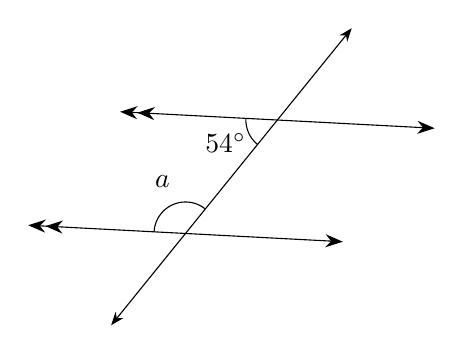
\begin{tikzpicture}[scale=1.0, baseline=(current bounding box.north)]
    \begin{scope}[rotate=51]
      % Draw the first line
      \draw[<->>, >={Stealth[scale=1.3]}, name path=P1] (0, 0) -- (-2.351141009169892, 3.23606797749979);
      % Draw the second line with the calculated offsets
      \draw[<->>, >={Stealth[scale=1.3]}, name path=P2] (1.8541019662496845, 0) -- (-0.4970390429202076, 3.23606797749979);
      % Draw the transversal through the middle of the parallel lines
      \draw[<->, >=Stealth, name path=P3] (-2.6755705045849463, 1.618033988749895) -- (2.1785314616647384, 1.618033988749895);
      
      \path [name intersections={of=P1 and P3,by=A}];
      \path [name intersections={of=P2 and P3,by=B}];

      % Draw the angle
      \coordinate (p1s) at (0, 0);
      \coordinate (p1e) at (-2.351141009169892, 3.23606797749979);
      \coordinate (p2s) at (1.8541019662496845, 0);
      \coordinate (p2e) at (-0.4970390429202076, 3.23606797749979);
      \coordinate (ts) at (-2.6755705045849463, 1.618033988749895);
      \coordinate (te) at (2.1785314616647384, 1.618033988749895);

      % order for vertices go in anticlockwise order te--A--p1e
      \draw pic["$a$", draw=black, -, angle eccentricity=1.8, angle radius=0.4cm] {angle=te--A--p1e};
\draw pic["$54^\circ$", draw=black, -, angle eccentricity=1.8, angle radius=0.4cm] {angle=p2e--B--ts};

      % %% Point A
      % \draw pic["$a$", draw=black, -, angle eccentricity=1.5, angle radius=0.4cm] {angle=te--A--p1e};
      % \draw pic["$b$", draw=black, -, angle eccentricity=1.5, angle radius=0.4cm] {angle=p1e--A--ts};
      % \draw pic["$c$", draw=black, -, angle eccentricity=1.5, angle radius=0.4cm] {angle=ts--A--p1s};
      % \draw pic["$d$", draw=black, -, angle eccentricity=1.5, angle radius=0.4cm] {angle=p1s--A--te};
      
      % %%  Point B
      % \draw pic["$e$", draw=black, -, angle eccentricity=1.5, angle radius=0.4cm] {angle=te--B--p2e};
      % \draw pic["$f$", draw=black, -, angle eccentricity=1.5, angle radius=0.4cm] {angle=p2e--B--ts};
      % \draw pic["$g$", draw=black, -, angle eccentricity=1.5, angle radius=0.4cm] {angle=ts--B--p2s};
      % \draw pic["$h$", draw=black, -, angle eccentricity=1.5, angle radius=0.4cm] {angle=p2s--B--te};

    \end{scope}
  \end{tikzpicture}
\end{minipage}%
\hfill
\begin{minipage}{0.2\textwidth}
  \begin{align*}
    \angle \text{a} &= \text{\dotuline{~~~~~~~}}^\circ
  \end{align*}
\end{minipage}
\vspace{1cm}\begin{minipage}{0.75\textwidth}
  \refstepcounter{minipagecount}
  \noindent{(\theminipagecount)}\quad
  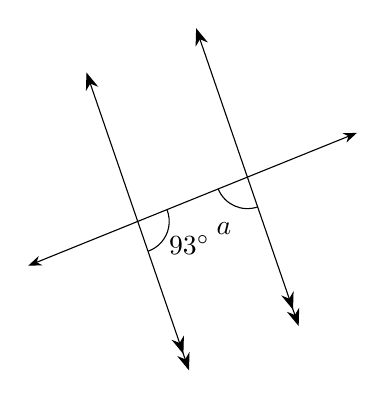
\begin{tikzpicture}[scale=1.0, baseline=(current bounding box.north)]
    \begin{scope}[rotate=202]
      % Draw the first line
      \draw[<->>, >={Stealth[scale=1.3]}, name path=P1] (0, 0) -- (0.20934382497177587, 3.9945181390182953);
      % Draw the second line with the calculated offsets
      \draw[<->>, >={Stealth[scale=1.3]}, name path=P2] (1.5020585189968816, 0) -- (1.7114023439686574, 3.9945181390182953);
      % Draw the transversal through the middle of the parallel lines
      \draw[<->, >=Stealth, name path=P3] (-1.395328087514112, 1.9972590695091477) -- (3.1067304314827697, 1.9972590695091477);
      
      \path [name intersections={of=P1 and P3,by=A}];
      \path [name intersections={of=P2 and P3,by=B}];

      % Draw the angle
      \coordinate (p1s) at (0, 0);
      \coordinate (p1e) at (0.20934382497177587, 3.9945181390182953);
      \coordinate (p2s) at (1.5020585189968816, 0);
      \coordinate (p2e) at (1.7114023439686574, 3.9945181390182953);
      \coordinate (ts) at (-1.395328087514112, 1.9972590695091477);
      \coordinate (te) at (3.1067304314827697, 1.9972590695091477);

      % order for vertices go in anticlockwise order te--A--p1e
      \draw pic["$a$", draw=black, -, angle eccentricity=1.8, angle radius=0.4cm] {angle=te--A--p1e};
\draw pic["$93^\circ$", draw=black, -, angle eccentricity=1.8, angle radius=0.4cm] {angle=p2e--B--ts};

      % %% Point A
      % \draw pic["$a$", draw=black, -, angle eccentricity=1.5, angle radius=0.4cm] {angle=te--A--p1e};
      % \draw pic["$b$", draw=black, -, angle eccentricity=1.5, angle radius=0.4cm] {angle=p1e--A--ts};
      % \draw pic["$c$", draw=black, -, angle eccentricity=1.5, angle radius=0.4cm] {angle=ts--A--p1s};
      % \draw pic["$d$", draw=black, -, angle eccentricity=1.5, angle radius=0.4cm] {angle=p1s--A--te};
      
      % %%  Point B
      % \draw pic["$e$", draw=black, -, angle eccentricity=1.5, angle radius=0.4cm] {angle=te--B--p2e};
      % \draw pic["$f$", draw=black, -, angle eccentricity=1.5, angle radius=0.4cm] {angle=p2e--B--ts};
      % \draw pic["$g$", draw=black, -, angle eccentricity=1.5, angle radius=0.4cm] {angle=ts--B--p2s};
      % \draw pic["$h$", draw=black, -, angle eccentricity=1.5, angle radius=0.4cm] {angle=p2s--B--te};

    \end{scope}
  \end{tikzpicture}
\end{minipage}%
\hfill
\begin{minipage}{0.2\textwidth}
  \begin{align*}
    \angle \text{a} &= \text{\dotuline{~~~~~~~}}^\circ
  \end{align*}
\end{minipage}
\vspace{1cm}\begin{minipage}{0.75\textwidth}
  \refstepcounter{minipagecount}
  \noindent{(\theminipagecount)}\quad
  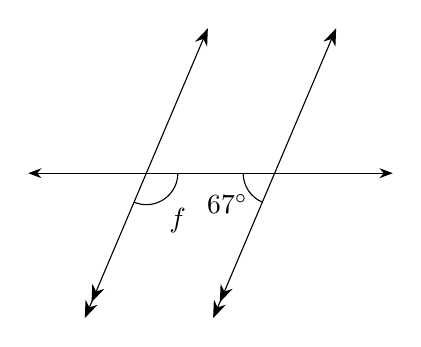
\begin{tikzpicture}[scale=1.0, baseline=(current bounding box.north)]
    \begin{scope}[rotate=180]
      % Draw the first line
      \draw[<->>, >={Stealth[scale=1.3]}, name path=P1] (0, 0) -- (1.5629245139570949, 3.6820194138097615);
      % Draw the second line with the calculated offsets
      \draw[<->>, >={Stealth[scale=1.3]}, name path=P2] (1.6295405661079443, 0) -- (3.1924650800650394, 3.6820194138097615);
      % Draw the transversal through the middle of the parallel lines
      \draw[<->, >=Stealth, name path=P3] (-0.7185377430214523, 1.8410097069048807) -- (3.9110028230864917, 1.8410097069048807);
      
      \path [name intersections={of=P1 and P3,by=A}];
      \path [name intersections={of=P2 and P3,by=B}];

      % Draw the angle
      \coordinate (p1s) at (0, 0);
      \coordinate (p1e) at (1.5629245139570949, 3.6820194138097615);
      \coordinate (p2s) at (1.6295405661079443, 0);
      \coordinate (p2e) at (3.1924650800650394, 3.6820194138097615);
      \coordinate (ts) at (-0.7185377430214523, 1.8410097069048807);
      \coordinate (te) at (3.9110028230864917, 1.8410097069048807);

      % order for vertices go in anticlockwise order te--A--p1e
      \draw pic["$f$", draw=black, -, angle eccentricity=1.8, angle radius=0.4cm] {angle=p2e--B--ts};
\draw pic["$67^\circ$", draw=black, -, angle eccentricity=1.8, angle radius=0.4cm] {angle=te--A--p1e};

      % %% Point A
      % \draw pic["$a$", draw=black, -, angle eccentricity=1.5, angle radius=0.4cm] {angle=te--A--p1e};
      % \draw pic["$b$", draw=black, -, angle eccentricity=1.5, angle radius=0.4cm] {angle=p1e--A--ts};
      % \draw pic["$c$", draw=black, -, angle eccentricity=1.5, angle radius=0.4cm] {angle=ts--A--p1s};
      % \draw pic["$d$", draw=black, -, angle eccentricity=1.5, angle radius=0.4cm] {angle=p1s--A--te};
      
      % %%  Point B
      % \draw pic["$e$", draw=black, -, angle eccentricity=1.5, angle radius=0.4cm] {angle=te--B--p2e};
      % \draw pic["$f$", draw=black, -, angle eccentricity=1.5, angle radius=0.4cm] {angle=p2e--B--ts};
      % \draw pic["$g$", draw=black, -, angle eccentricity=1.5, angle radius=0.4cm] {angle=ts--B--p2s};
      % \draw pic["$h$", draw=black, -, angle eccentricity=1.5, angle radius=0.4cm] {angle=p2s--B--te};

    \end{scope}
  \end{tikzpicture}
\end{minipage}%
\hfill
\begin{minipage}{0.2\textwidth}
  \begin{align*}
    \angle \text{f} &= \text{\dotuline{~~~~~~~}}^\circ
  \end{align*}
\end{minipage}
\vspace{1cm}

\end{document}
